\documentclass[12pt,a4paper]{article}

\usepackage[french]{babel}
\usepackage[utf8]{inputenc}
\usepackage[T1]{fontenc}

\usepackage{tikz}
\usetikzlibrary{calc}

\usepackage{geometry}
\geometry{margin=1in}

\usepackage{listings}
\usepackage{courier}

\lstdefinelanguage{Isabelle}{
  morekeywords={theory,imports,begin,end,definition,lemma,theorem,proof,qed,
    assumes,shows,fixes,defines,datatype,record,fun,primrec,abbreviation,
    axiomatization,where,using,by,unfolding},
  sensitive=true,
  morecomment=[s]{(*}{*)},
  morestring=[b]"
}

\lstset{
  language=Isabelle,
  basicstyle=\ttfamily\small,
  keywordstyle=\bfseries,
  commentstyle=\itshape\color{gray},
  columns=fullflexible,
  keepspaces=true,
  showstringspaces=false,
}
\usepackage{listings}
\usepackage{xcolor}
\usepackage{courier}

% Couleur gris pâle pour l'encadre
\definecolor{lightgray}{gray}{0.95}

% Definition du style Isabelle dans un encadre gris
\lstdefinelanguage{Isabelle}{
  morekeywords={theory,imports,begin,end,definition,lemma,theorem,proof,qed,
    assumes,shows,fixes,defines,datatype,record,fun,primrec,abbreviation,
    axiomatization,where,using,by,unfolding},
  sensitive=true,
  morecomment=[s]{(*}{*)},
  morestring=[b]"
}

\lstdefinestyle{isabellegray}{
  language=Isabelle,
  backgroundcolor=\color{lightgray},
  basicstyle=\ttfamily\small,
  keywordstyle=\bfseries,
  commentstyle=\itshape\color{gray},
  frame=single,
  rulecolor=\color{black},
  columns=fullflexible,
  keepspaces=true,
  showstringspaces=false,
  breaklines=true,
  breakatwhitespace=true
}
\begin{document}

% ============================================================
% PAGE TITRE
% ============================================================

\begin{titlepage}
    \centering

    {\Huge \textbf{Mecanique harmonique du chaos discret}}\\[1.5cm]

    {\Large \textbf{Auteur :} Philippe Thomas Savard}\\[0.3cm]
    {\large Levis, Chaudiere-Appalaches, Canada}\\[0.8cm]

    {\large \textbf{Licence :} Apache 2.0}\\[0.8cm]

    {\large \textbf{Date :} Le huit mars deux mille vingt-six}\\[2cm]

    \vfill
\end{titlepage}

% ============================================================
% PREFACE
% ============================================================

\vspace{0.5cm}

Ce document a ete redige sans financement, sans avantages materiels ou symboliques, 
et dans une totale liberte de conscience et de jugement. 
Ce texte est le fruit d'une experience de pensee, illustree par des calculs mathematiques, 
des schemas, des tableaux, ainsi que des exemples et explications. 
L'auteur n'est pas initie aux mathematiques au sens academique : 
il ne possede aucune formation specialisee dans ce domaine. 
Il est ouvrier, et c'est en dehors des sentiers balises qu'il a conçu ce document 
par pur plaisir intellectuel et en consequence d'un interet profond pour les mathematiques.

\vspace{0.5cm}

% ============================================================
% SECTION : FIGURE
% ============================================================

\section*{Figure de la mecanique harmonique du chaos discret}

Cette figure est le schema sur lequel l'auteur applique un raisonnement intuitif 
qui lui permet de determiner la possibilite d'une invariance geometrique nouvelle. 
Cette invariance est relative, tout comme la relativite ou la position de l'observateur 
influence la mesure. Dans la mecanique harmonique du chaos discret, 
c'est l'unite choisie qui influence la mesure.

L'auteur trace un parallele avec la constante d'Euler-Mascheroni, 
ou plutôt avec l'interet lie à l'exactitude de cette constante, 
qui devient plus precise à la quatrieme decimale lorsqu'elle est interpretee 
en sens contraire de la lecture habituelle. 
La constante d'Euler-Mascheroni, qu'il simplifie à la forme 
\(0.5 / \sin 60^\circ\), est evoquee dans l'equation lui permettant 
de determiner l'unite. Il emprunte une approche originale pour determiner 
l'unite choisie par le produit du diametre du carre AEFG 
par le rapport entre 0.5 et le resultat de l'arcsin de LM, 
soit : \texttt{AEFG * (0.5 / sin(angle))}.

\vspace{0.8cm}

% ============================================================
% FIGURE TIKZ COMPLETE
% ============================================================

\begin{tikzpicture}[scale=1.8]

% Couleurs
\definecolor{grisA}{gray}{0.55}
\definecolor{grisB}{gray}{0.45}
\definecolor{grisC}{gray}{0.35}

\pgfmathsetmacro{\rtthree}{sqrt(3)}

% Carre principal ABCD (2.25)
\coordinate (A) at (0,0);
\coordinate (B) at (2.25,0);
\coordinate (C) at (2.25,2.25);
\coordinate (D) at (0,2.25);

% Carre interieur AEFG (1.5)
\coordinate (E) at (1.5,0);
\coordinate (F) at (1.5,1.5);
\coordinate (G) at (0,1.5);

% Quadrillage fractal
\foreach \x in {0,0.5,...,2.25}
  \foreach \y in {0,0.5,...,2.25}
    \draw[grisA!70,thin] (\x,\y) rectangle ++(0.5,0.5);

\foreach \x in {0,0.25,...,3.375}
  \foreach \y in {0,0.25,...,3.375}
    {
      \ifdim\x pt<2.25pt
        \ifdim\y pt<2.25pt
        \else
          \draw[grisB!55,thin] (\x,\y) rectangle ++(0.25,0.25);
        \fi
      \else
        \draw[grisB!55,thin] (\x,\y) rectangle ++(0.25,0.25);
      \fi
    }

\foreach \x in {0,0.125,...,5.0625}
  \foreach \y in {0,0.125,...,5.0625}
    {
      \ifdim\x pt<3.375pt
        \ifdim\y pt<3.375pt
        \else
          \draw[grisC!45,thin] (\x,\y) rectangle ++(0.125,0.125);
        \fi
      \else
        \draw[grisC!45,thin] (\x,\y) rectangle ++(0.125,0.125);
      \fi
    }

% Carres
\draw[thick] (A)--(B)--(C)--(D)--cycle;
\draw[thick] (A)--(E)--(F)--(G)--cycle;

% Triangles equilateraux inscrits (jaune et vert)
\pgfmathsetmacro{\aC}{2.25/(\rtthree + 0.5)}
\coordinate (H) at (\aC,0);
\coordinate (I) at (0,\aC);
\filldraw[yellow!60, draw=black, thick] (C)--(H)--(I)--cycle;

\pgfmathsetmacro{\aF}{1.5/(\rtthree + 0.5)}
\coordinate (J) at (\aF,0);
\coordinate (K) at (0,\aF);
\filldraw[green!60, draw=black, thick] (F)--(J)--(K)--cycle;

% Triangles supplementaires (contours gris pale)
\pgfmathsetmacro{\aThree}{3.375/(\rtthree + 0.5)}
\coordinate (C3) at (3.375,3.375);
\coordinate (H3) at (\aThree,0);
\coordinate (I3) at (0,\aThree);
\draw[gray!60, thick] (C3)--(H3)--(I3)--cycle;

\pgfmathsetmacro{\aFour}{5.0625/(\rtthree + 0.5)}
\coordinate (C4) at (5.0625,5.0625);
\coordinate (H4) at (\aFour,0);
\coordinate (I4) at (0,\aFour);
\draw[gray!50, thick] (C4)--(H4)--(I4)--cycle;

% Diametres AC et AF
\draw[gray!60,thick] (A)--(C);
\draw[gray!60,thick] (A)--(F);

% Points L et M
\coordinate (L) at ({0.5*\aF},{0.5*\aF});
\coordinate (M) at ({0.5*\aC},{0.5*\aC});

\draw[blue,thick] (A)--(L);
\draw[red,thick] (L)--(M);
\draw[blue,thick] (M)--(C);

% Etiquettes
\foreach \P in {A,B,C,D,E,F,G,H,I,J,K}
  \node[black] at (\P) [shift={(0.12,0.12)}] {$\P$};

\node at (L) [above left] {$L$};
\node at (M) [above left] {$M$};

\end{tikzpicture}
\begin{figure}[h!]
    \centering
    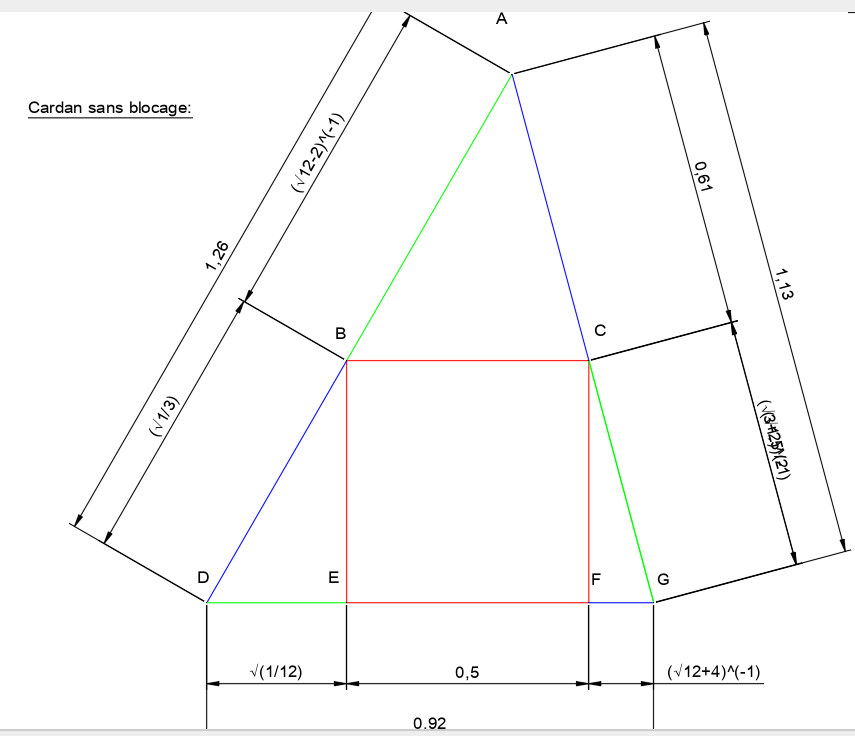
\includegraphics[width=0.85\textwidth]{cardan_blocage.png}
    \caption{Cardan sans blocage - version de reference}
    \label{fig:cardan_blocage}
\end{figure}

% ============================================================
% SECTION : SCRIPT ISABELLE HOL
% ============================================================

\section*{Script Isabelle HOL : mecanique\_discret.thy}

Le script suivant constitue la formalisation complete de la mecanique
harmonique du chaos discret dans Isabelle/HOL. Il a ete valide par le
moteur de preuve et compile sans erreur via :

\texttt{isabelle build -D .}

\begin{lstlisting}[style=isabellegray]
theory mecanique_discret
  imports Complex_Main
begin

(theory mecanique_discret
  imports Complex_Main
begin


subsection "A1.0 Axiomatisation de la mecanique harmonique du chaos discret"

text "
  La configuration geometrique fondamentale repose sur une famille de carres
  emboîtes, tous alignes avec les axes du plan cartesien et partageant le point
  commun A = (0,0). Le carre de niveau n possede un cote de longueur 1.5^n,
  ce qui correspond exactement aux elevations visibles dans la figure TikZ :

      1.5^1, 1.5^2, 1.5^3, 1.5^4, ..., 1.5^n.

  Dans chaque carre de niveau n est inscrit un triangle isocele dont le sommet
  superieur est le point C(n) = (1.5^n, 1.5^n), et dont la base repose sur les
  axes de coordonnees. La base est constituee des deux points :

      P1(n,p) = (b(n,p), 0)
      P2(n,p) = (0, b(n,p))

  ou b(n,p) est une longueur strictement positive dependant du niveau n et du
  nombre premier p.

  Lorsque la diagonale AC(n) coupe la base du triangle inscrit, celui-ci est
  divise en deux triangles rectangles. Dans chacun de ces triangles rectangles,
  la demi-base vaut b(n,p)/2 et la hauteur vaut h(n,p). Le rapport geometrique
  fondamental de la mecanique harmonique du chaos discret est :

      (b(n,p) / 2) / h(n,p) = sqrt(p)

  ou p est un nombre premier definissant l'unite admissible.

  Ce rapport ne concerne donc pas le triangle complet, mais le demi-triangle
  rectangle issu de la coupure par la diagonale AC(n). Ce point est essentiel :
  c'est ce demi-triangle rectangle qui porte l'information geometrique
  fondamentale de l'unite p.

  Le rapport ci-dessus determine l'angle θ(p) du triangle rectangle par :

      tan(θ(p)) = sqrt(p)
      θ(p) = arctan(sqrt(p))

  Cet angle joue un role central dans les chapitres B et C, notamment dans la
  matrice à derive premiere et dans la structure du prisme matriciel.
"

subsubsection "A1.1 Unites admissibles"

definition prime_nat :: "nat ⇒ bool" where
  "prime_nat p ⟷ (p > 1 ∧ (∀m. m dvd p ⟶ m = 1 ∨ m = p))"

definition admissible_unit :: "nat ⇒ bool" where
  "admissible_unit p ⟷ prime_nat p"

definition unit :: "nat ⇒ real" where
  "unit p = sqrt (real p) + 1"

subsubsection "A1.2 Carres emboîtes"

type_synonym point = "real × real"

definition side :: "nat ⇒ real" where
  "side n = (1.5 :: real) ^ n"

definition A :: point where "A = (0,0)"
definition B :: "nat ⇒ point" where "B n = (side n, 0)"
definition C :: "nat ⇒ point" where "C n = (side n, side n)"
definition D :: "nat ⇒ point" where "D n = (0, side n)"

subsubsection "A1.3 Triangles inscrits"

text "
  Le triangle inscrit dans le carre de niveau n et associe à l'unite p possede
  les sommets :

      C(n), P1(n,p), P2(n,p)

  ou la base repose sur les axes et le sommet est C(n).
"

definition base_param :: "nat ⇒ nat ⇒ real" where
  "base_param n p = (side n) / (sqrt (real p) + 0.5)"

definition P1 :: "nat ⇒ nat ⇒ point" where
  "P1 n p = (base_param n p, 0)"

definition P2 :: "nat ⇒ nat ⇒ point" where
  "P2 n p = (0, base_param n p)"

subsubsection "A1.4 Rapport fondamental : demi-base / hauteur = sqrt(p)"

definition dist2 :: "point ⇒ point ⇒ real" where
  "dist2 P Q = sqrt ((fst P - fst Q)^2 + (snd P - snd Q)^2)"

definition base_length :: "nat ⇒ nat ⇒ real" where
  "base_length n p = dist2 (P1 n p) (P2 n p)"

definition height_length :: "nat ⇒ nat ⇒ real" where
  "height_length n p =
     abs ((2 * side n - base_param n p) / sqrt 2)"

definition ratio_halfbase_height :: "nat ⇒ nat ⇒ real" where
  "ratio_halfbase_height n p =
     ((base_length n p) / 2) / (height_length n p)"

axiomatization where
  ratio_axiom:
    "⟦ admissible_unit p; n ≥ 1 ⟧
     ⟹ ratio_halfbase_height n p = sqrt (real p)"
subsubsection "A1.5 Angle associe à l'unite p"

definition angle_rect :: "nat ⇒ real" where
  "angle_rect p = arctan (sqrt (real p))"


subsection "B2.0 Angle oppose dans le demi-triangle rectangle"

text "
  Lorsque la diagonale AC coupe la base du triangle inscrit, celui-ci est divise
  en deux triangles rectangles. Dans chacun de ces triangles rectangles, la
  demi-base vaut b/2 et la hauteur vaut h. Le rapport geometrique fondamental est :

      (b / 2) / h = sqrt(p)

  L'angle oppose a la demi-base est donc :

      θ(p) = arctan(sqrt(p))

  Cette fonction joue un role central dans la matrice à derive premiere.
"


subsection "B2.1 Angle oppose pour la matrice à derive premiere"

text "
  Nous reutilisons la fonction angle_rect definie dans le Chapitre A.
  Elle encode l'angle du demi-triangle rectangle associe à l'unite p.
"

lemma angle_rect_prime:
  assumes "prime_nat p"
  shows "angle_rect p = arctan (sqrt (real p))"
  by (simp add: angle_rect_def)


subsubsection "A1.6 Unite geometrique via le segment AL_nat"

text "
  On definit le segment AL_nat(p) de maniere à ce que l'unite geometrique :

      U(p) = √4.5 / AL_nat(p)

  soit egale à l'unite abstraite √p + 1.

  On obtient :

      AL_nat(p) = √4.5 / (√p + 1).
"

definition AL_nat :: "nat ⇒ real" where
  "AL_nat p = sqrt 4.5 / (sqrt (real p) + 1)"

definition geometric_unit :: "nat ⇒ real" where
  "geometric_unit p = sqrt 4.5 / AL_nat p"


lemma geometric_unit_eq_unit:
  assumes "AL_nat p ≠ 0"
  shows "geometric_unit p = sqrt (real p) + 1"
proof -
  have "geometric_unit p = sqrt 4.5 / AL_nat p"
    by (simp add: geometric_unit_def)
  also have "... = sqrt 4.5 / (sqrt 4.5 / (sqrt (real p) + 1))"
    by (simp add: AL_nat_def)
  also have "... = sqrt (real p) + 1"
    using assms by (simp add: field_simps)
  finally show ?thesis .
qed


axiomatization where
  AL_nat_domain:
    "admissible_unit p ⟹ AL_nat p ≠ 0"
subsubsection "A1.6 Axiome d'invariance (version demontree)"

text "
  Pour toute unite admissible p, l'unite geometrique definie par AL_nat(p)
  coincide avec l'unite abstraite √p + 1.
"

(* Definition correcte de l'unite abstraite *)
definition u_nat :: "nat ⇒ real" where
  "u_nat p = sqrt (real p) + 1"

lemma invariance_geometric_unit:
  assumes "admissible_unit p"
  shows "geometric_unit p = u_nat p"
proof -
  have "AL_nat p ≠ 0"
    using assms AL_nat_domain by blast
  hence "geometric_unit p = sqrt (real p) + 1"
    using geometric_unit_eq_unit by blast
  thus ?thesis
    by (simp add: u_nat_def)
qed


subsection "B1.0 Cardan sans blocage (formalise)"

definition pol :: "real ⇒ real ⇒ point" where
  "pol r θ = (r * cos θ, r * sin θ)"

definition ang_BDE :: real where "ang_BDE = (pi / 3)"     (* 60° *)
definition ang_CGF :: real where "ang_CGF = (5*pi / 12)"  (* 75° *)
definition ang_BAC :: real where "ang_BAC = (pi / 4)"     (* 45° *)

definition BD_len :: real where "BD_len = sqrt (1/3)"
definition DE_len :: real where "DE_len = sqrt (1/12)"
definition BC_len :: real where "BC_len = 0.5"
definition EF_len :: real where "EF_len = 0.5"
definition FG_len :: real where "FG_len = 1 / (sqrt (12 :: real) + 4)"
definition CG_len :: real where "CG_len = 1 / (sqrt (3 :: real) + 2)"
definition AB_len :: real where "AB_len = 1 / (sqrt (12 :: real) - 2)"
definition AC_len :: real where "AC_len = sqrt (1.5 :: real) / 2"
definition DG_len :: real where "DG_len = 1.26"
definition AG_len :: real where "AG_len = 1.13"

definition card_D :: point where "card_D = (0,0)"
definition card_G :: point where "card_G = pol DG_len 0"
definition card_A :: point where "card_A = pol AG_len ang_BDE"
definition card_B :: point where "card_B = pol BD_len ang_BDE"
definition card_E :: point where "card_E = pol DE_len (ang_BDE + ang_BDE)"
definition card_C :: point where "card_C = pol AC_len (ang_BDE - ang_BAC)"
definition card_F :: point where "card_F = pol EF_len (ang_BDE - ang_BAC + (pi/2))"
definition card_G2 :: point where "card_G2 = pol CG_len (ang_BDE - ang_BAC - ang_CGF)"


chapter C
section ‹C1.0 Matrice a derive premiere›

text "
  Formalisation de la matrice à derive premiere associee au cardan sans blocage.
"

type_synonym length = real

record cardan_lengths =
  AD      :: length
  AB      :: length
  BD      :: length
  AG      :: length
  AC      :: length
  CG      :: length
  DG      :: length
  EF      :: length
  DE      :: length
  FG      :: length
  diam_eq :: real
  u15     :: real
  u3375   :: real

definition C1 :: "cardan_lengths ⇒ length" where "C1 L = AD L"
definition C2 :: "cardan_lengths ⇒ length" where "C2 L = AB L"
definition C3 :: "cardan_lengths ⇒ length" where "C3 L = BD L"
definition C4 :: "cardan_lengths ⇒ length" where "C4 L = AG L"
definition C5 :: "cardan_lengths ⇒ length" where "C5 L = AC L"
definition C6 :: "cardan_lengths ⇒ length" where "C6 L = CG L"
definition C7 :: "cardan_lengths ⇒ length" where "C7 L = DG L"
definition C8 :: "cardan_lengths ⇒ length" where "C8 L = EF L"
definition C9 :: "cardan_lengths ⇒ length" where "C9 L = DE L + FG L"

definition R1 :: "cardan_lengths ⇒ length" where
  "R1 L = C1 L + C2 L + C3 L"

definition R2 :: "cardan_lengths ⇒ length" where
  "R2 L = C4 L + C5 L + C6 L"

definition R3 :: "cardan_lengths ⇒ length" where
  "R3 L = C7 L + C8 L + C9 L"


subsection "1. Matrice deduite des mesures du plan"

definition M1_L1 :: "cardan_lengths ⇒ bool" where
  "M1_L1 L ⟷
     C1 L * diam_eq L + C2 L * diam_eq L + C3 L * diam_eq L
       = 2 * C1 L * diam_eq L"

definition M1_L2 :: "cardan_lengths ⇒ bool" where
  "M1_L2 L ⟷
     C4 L * u15 L + C5 L * u15 L + C6 L * u15 L
       = 2 * C4 L * u15 L"

definition M1_L3 :: "cardan_lengths ⇒ bool" where
  "M1_L3 L ⟷
     C7 L * u3375 L + C8 L * u3375 L + C9 L * u3375 L
       = 2 * C7 L * u3375 L"

definition M1_matrix :: "cardan_lengths ⇒ bool" where
  "M1_matrix L ⟷ M1_L1 L ∧ M1_L2 L ∧ M1_L3 L"


subsection "2. Matrice de transition"

record drift_transition =
  C1'  :: real
  C2'  :: real
  C3'  :: real
  C4'  :: real
  C5'  :: real
  C6'  :: real
  C7'  :: real
  C8'  :: real
  C9'  :: real
  R1'  :: real
  R2'  :: real
  R3'  :: real
  diam_eq' :: real
  u15'     :: real
  u3375'   :: real
text "
  Structure de la matrice de transition :

    C1' + C2' + C3' = R1'
    C4' + C5' + C6' = R2'
    C7' + C8' + C9' = R3'

    R1' = 2 * C1' * diam_eq'
    R2' = 2 * C3' * u15'
    R3' = 2 * C6' * u3375'
"
definition M2_structure :: "drift_transition ⇒ bool" where
  "M2_structure T ⟷
     C1' T + C2' T + C3' T = R1' T ∧
     C4' T + C5' T + C6' T = R2' T ∧
     C7' T + C8' T + C9' T = R3' T ∧
     R1' T = 2 * C1' T * diam_eq' T ∧
     R2' T = 2 * C3' T * u15' T ∧
     R3' T = 2 * C6' T * u3375' T"


subsection "3. Matrice à derive premiere simplifiee"

text "
  Matrice simplifiee (nombres premiers) :

    L1 : 37x + 31x + 29x = 41x
    L2 : 19y + 17y + 13y = 23y
    L3 :  7z +  5z +  3z = 11z

  Version ponderee avec l'inconnue unique u = sqrt 3.375 :

    L1 : 37 (7/48.5) u + 31 (7/48.5) u + 29 (7/48.5) u = 41 (7/20.5) u
    L2 : 19 (7/24.5) u + 17 (7/24.5) u + 13 (7/24.5) u = 23 (7/11.5) u
    L3 :  7 (7/7.5)  u +  5 (7/7.5)  u +  3 (7/7.5)  u = 11 (7/5.5)  u
"

definition u :: real where
  "u = sqrt (3.375 :: real)"

definition L1_simplified :: "real ⇒ bool" where
  "L1_simplified x ⟷ 37*x + 31*x + 29*x = 41*x"

definition L2_simplified :: "real ⇒ bool" where
  "L2_simplified y ⟷ 19*y + 17*y + 13*y = 23*y"

definition L3_simplified :: "real ⇒ bool" where
  "L3_simplified z ⟷ 7*z + 5*z + 3*z = 11*z"

definition L1_weighted :: bool where
  "L1_weighted ⟷
     37 * (7/48.5) * u +
     31 * (7/48.5) * u +
     29 * (7/48.5) * u =
     41 * (7/20.5) * u"

definition L2_weighted :: bool where
  "L2_weighted ⟷
     19 * (7/24.5) * u +
     17 * (7/24.5) * u +
     13 * (7/24.5) * u =
     23 * (7/11.5) * u"

definition L3_weighted :: bool where
  "L3_weighted ⟷
     7 * (7/7.5) * u +
     5 * (7/7.5) * u +
     3 * (7/7.5) * u =
     11 * (7/5.5) * u"

definition M3_matrix :: bool where
  "M3_matrix ⟷ L1_weighted ∧ L2_weighted ∧ L3_weighted"


text "
-------------------------------------------------------------------------------
                           CREDITS ET LICENCE
-------------------------------------------------------------------------------

Titre  : Mecanique harmonique du chaos discret
Auteur : Philippe Thomas Savard
Date   : 10 mars 2026
Lieu   : Levis, Chaudieres-Appalaches, Canada

Ce travail est distribue sous la licence Apache 2.0.

-------------------------------------------------------------------------------
LICENCE APACHE 2.0 (TEXTE COMPLET)
-------------------------------------------------------------------------------

                                 Apache License
                           Version 2.0, January 2004
                        http://www.apache.org/licenses/

TERMS AND CONDITIONS FOR USE, REPRODUCTION, AND DISTRIBUTION

1. Definitions.

   \"License\" shall mean the terms and conditions for use, reproduction,
   and distribution as defined by Sections 1 through 9 of this document.

   \"Licensor\" shall mean the copyright owner or entity authorized by
   the copyright owner that is granting the License.

   \"Legal Entity\" shall mean the union of the acting entity and all
   other entities that control, are controlled by, or are under common
   control with that entity. For the purposes of this definition,
   \"control\" means (i) the power, direct or indirect, to cause the
   direction or management of such entity, whether by contract or
   otherwise, or (ii) ownership of fifty percent (50%) or more of the
   outstanding shares, or (iii) beneficial ownership of such entity.

   \"You\" (or \"Your\") shall mean an individual or Legal Entity
   exercising permissions granted by this License.

   \"Source\" form shall mean the preferred form for making modifications,
   including but not limited to software source code, documentation source,
   and configuration files.

   \"Object\" form shall mean any form resulting from mechanical
   transformation or translation of a Source form, including but not
   limited to compiled object code, generated documentation, and
   conversions to other media types.

   \"Work\" shall mean the work of authorship, whether in Source or
   Object form, made available under the License, as indicated by a
   copyright notice that is included in or attached to the work.

   \"Derivative Works\" shall mean any work, whether in Source or Object
   form, that is based on (or derived from) the Work and for which the
   editorial revisions, annotations, elaborations, or other modifications
   represent, as a whole, an original work of authorship. For the purposes
   of this License, Derivative Works shall not include works that remain
   separable from, or merely link (or bind by name) to the interfaces of,
   the Work and Derivative Works thereof.

   \"Contribution\" shall mean any work of authorship, including the
   original version of the Work and any modifications or additions to
   that Work or Derivative Works thereof, that is intentionally submitted
   to Licensor for inclusion in the Work by the copyright owner or by an
   individual or Legal Entity authorized to submit on behalf of the
   copyright owner.

   \"Contributor\" shall mean Licensor and any individual or Legal Entity
   on behalf of whom a Contribution has been received by Licensor and
   subsequently incorporated within the Work.

2. Grant of Copyright License.

   Subject to the terms and conditions of this License, each Contributor
   hereby grants to You a perpetual, worldwide, non-exclusive, no-charge,
   royalty-free, irrevocable copyright license to reproduce, prepare
   Derivative Works of, publicly display, publicly perform, sublicense,
   and distribute the Work and such Derivative Works in Source or Object
   form.

3. Grant of Patent License.

   Subject to the terms and conditions of this License, each Contributor
   hereby grants to You a perpetual, worldwide, non-exclusive, no-charge,
   royalty-free, irrevocable (except as stated in this section) patent
   license to make, have made, use, offer to sell, sell, import, and
   otherwise transfer the Work.

4. Redistribution.

   You may reproduce and distribute copies of the Work or Derivative
   Works thereof in any medium, with or without modifications, and in
   Source or Object form, provided that You meet the following conditions:

   (a) You must give any other recipients of the Work a copy of this
       License; and

   (b) You must cause any modified files to carry prominent notices
       stating that You changed the files; and

   (c) You must retain, in the Source form of any Derivative Works that
       You distribute, all copyright, patent, trademark, and attribution
       notices from the Source form of the Work.

5. Submission of Contributions.

   Unless You explicitly state otherwise, any Contribution intentionally
   submitted for inclusion in the Work shall be under the terms and
   conditions of this License.

6. Trademarks.

   This License does not grant permission to use the trade names,
   trademarks, service marks, or product names of the Licensor.

7. Disclaimer of Warranty.

   Unless required by applicable law or agreed to in writing, Licensor
   provides the Work (and each Contributor provides its Contributions)
   on an \"AS IS\" BASIS, WITHOUT WARRANTIES OR CONDITIONS OF ANY KIND.

8. Limitation of Liability.

   In no event and under no legal theory shall any Contributor be liable
   to You for damages, including any direct, indirect, special,
   incidental, or consequential damages.

9. Accepting Warranty or Additional Liability.

   While redistributing the Work, You may choose to offer support or
   warranty protection for a fee, but You must do so on Your own behalf.

END OF TERMS AND CONDITIONS

-------------------------------------------------------------------------------
"
end
)

end
\end{lstlisting}

\end{document}